% Options for packages loaded elsewhere
\PassOptionsToPackage{unicode}{hyperref}
\PassOptionsToPackage{hyphens}{url}
%
\documentclass[
  ignorenonframetext,
]{beamer}
\title{Measuring Performance in Classification Models}
\author{}
\date{\vspace{-2.5em}}

\usepackage{pgfpages}
\setbeamertemplate{caption}[numbered]
\setbeamertemplate{caption label separator}{: }
\setbeamercolor{caption name}{fg=normal text.fg}
\beamertemplatenavigationsymbolsempty
% Prevent slide breaks in the middle of a paragraph
\widowpenalties 1 10000
\raggedbottom
\setbeamertemplate{part page}{
  \centering
  \begin{beamercolorbox}[sep=16pt,center]{part title}
    \usebeamerfont{part title}\insertpart\par
  \end{beamercolorbox}
}
\setbeamertemplate{section page}{
  \centering
  \begin{beamercolorbox}[sep=12pt,center]{part title}
    \usebeamerfont{section title}\insertsection\par
  \end{beamercolorbox}
}
\setbeamertemplate{subsection page}{
  \centering
  \begin{beamercolorbox}[sep=8pt,center]{part title}
    \usebeamerfont{subsection title}\insertsubsection\par
  \end{beamercolorbox}
}
\AtBeginPart{
  \frame{\partpage}
}
\AtBeginSection{
  \ifbibliography
  \else
    \frame{\sectionpage}
  \fi
}
\AtBeginSubsection{
  \frame{\subsectionpage}
}
\usepackage{amsmath,amssymb}
\usepackage{lmodern}
\usepackage{iftex}
\ifPDFTeX
  \usepackage[T1]{fontenc}
  \usepackage[utf8]{inputenc}
  \usepackage{textcomp} % provide euro and other symbols
\else % if luatex or xetex
  \usepackage{unicode-math}
  \defaultfontfeatures{Scale=MatchLowercase}
  \defaultfontfeatures[\rmfamily]{Ligatures=TeX,Scale=1}
\fi
% Use upquote if available, for straight quotes in verbatim environments
\IfFileExists{upquote.sty}{\usepackage{upquote}}{}
\IfFileExists{microtype.sty}{% use microtype if available
  \usepackage[]{microtype}
  \UseMicrotypeSet[protrusion]{basicmath} % disable protrusion for tt fonts
}{}
\makeatletter
\@ifundefined{KOMAClassName}{% if non-KOMA class
  \IfFileExists{parskip.sty}{%
    \usepackage{parskip}
  }{% else
    \setlength{\parindent}{0pt}
    \setlength{\parskip}{6pt plus 2pt minus 1pt}}
}{% if KOMA class
  \KOMAoptions{parskip=half}}
\makeatother
\usepackage{xcolor}
\IfFileExists{xurl.sty}{\usepackage{xurl}}{} % add URL line breaks if available
\IfFileExists{bookmark.sty}{\usepackage{bookmark}}{\usepackage{hyperref}}
\hypersetup{
  pdftitle={Measuring Performance in Classification Models},
  hidelinks,
  pdfcreator={LaTeX via pandoc}}
\urlstyle{same} % disable monospaced font for URLs
\newif\ifbibliography
\usepackage{longtable,booktabs,array}
\usepackage{calc} % for calculating minipage widths
\usepackage{caption}
% Make caption package work with longtable
\makeatletter
\def\fnum@table{\tablename~\thetable}
\makeatother
\usepackage{graphicx}
\makeatletter
\def\maxwidth{\ifdim\Gin@nat@width>\linewidth\linewidth\else\Gin@nat@width\fi}
\def\maxheight{\ifdim\Gin@nat@height>\textheight\textheight\else\Gin@nat@height\fi}
\makeatother
% Scale images if necessary, so that they will not overflow the page
% margins by default, and it is still possible to overwrite the defaults
% using explicit options in \includegraphics[width, height, ...]{}
\setkeys{Gin}{width=\maxwidth,height=\maxheight,keepaspectratio}
% Set default figure placement to htbp
\makeatletter
\def\fps@figure{htbp}
\makeatother
\setlength{\emergencystretch}{3em} % prevent overfull lines
\providecommand{\tightlist}{%
  \setlength{\itemsep}{0pt}\setlength{\parskip}{0pt}}
\setcounter{secnumdepth}{-\maxdimen} % remove section numbering
\usepackage{graphicx}
\usepackage{tikzpagenodes}
\usetikzlibrary{calc}
\usepackage{caption}
\ifLuaTeX
  \usepackage{selnolig}  % disable illegal ligatures
\fi

\begin{document}
\frame{\titlepage}

\begin{frame}
author: Son Nguyen
\end{frame}

\begin{frame}{Reading Materials}
\protect\hypertarget{reading-materials}{}
\begin{itemize}
\tightlist
\item
  Max Kuhn. Chapter 11.
\end{itemize}
\end{frame}

\begin{frame}{Two outcomes of classification models}
\protect\hypertarget{two-outcomes-of-classification-models}{}
\begin{itemize}
\tightlist
\item
  Predicted Probabilities
\item
  Class Prediction
\end{itemize}
\end{frame}

\begin{frame}{Examples}
\protect\hypertarget{examples}{}
\begin{itemize}
\tightlist
\item
  Predicting if a passenger in the titanic is survived or not survived
\item
  The outcome could look like this.
\end{itemize}

\begin{longtable}[]{@{}rll@{}}
\toprule
ID & Prob. of Survived & Prediction \\
\midrule
\endhead
1 & 0.55 & Survived \\
2 & 0.2 & Not Survived \\
3 & 0.94 & Survived \\
4 & 0.63 & Survived \\
5 & 0.9 & Survived \\
6 & 0.35 & Not Survived \\
7 & 0.84 & Survived \\
8 & 0.38 & Not Survived \\
9 & 0.01 & Not Survived \\
10 & 0.68 & Survived \\
11 & 0.71 & Survived \\
12 & 0.45 & Not Survived \\
\bottomrule
\end{longtable}
\end{frame}

\begin{frame}{Examples}
\protect\hypertarget{examples-1}{}
\begin{itemize}
\tightlist
\item
  Notice that this model predicts ``Survived'' for passengers with the
  probabilities of being greater than 0.5
\item
  0.5 is called \textbf{cut-off value}.
\item
  The cuff-off value is set by 0.5 by default.
\item
  The cut-off value can be changed by the modeler.
\end{itemize}
\end{frame}

\begin{frame}{Confusion Matrices}
\protect\hypertarget{confusion-matrices}{}
\begin{longtable}[]{@{}lll@{}}
\toprule
& Predicted Positive & Predicted Negative \\
\midrule
\endhead
\textbf{Actual Positive} & True Positive (TP) & False Negative (FN) \\
\textbf{Actual Negative} & False Positive (FP) & True Negative (TN) \\
\bottomrule
\end{longtable}
\end{frame}

\begin{frame}{Confusion Matrices}
\protect\hypertarget{confusion-matrices-1}{}
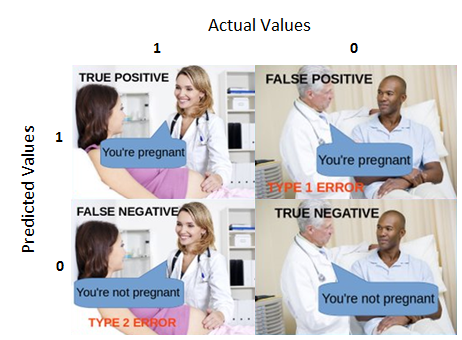
\includegraphics{images/cm.png}
\end{frame}

\begin{frame}{Confusion Matrices - Example}
\protect\hypertarget{confusion-matrices---example}{}
\begin{itemize}
\tightlist
\item
  ``Survived'' = \textbf{``Positive''}
\item
  ``Not Survived'' = \textbf{``Negative''}
\end{itemize}

\begin{longtable}[]{@{}rllll@{}}
\toprule
ID & Prob. of Survived & Prediction & Truth & Evaluation \\
\midrule
\endhead
1 & 0.55 & Survived & Survived & TP \\
2 & 0.2 & Not Survived & Survived & FN \\
3 & 0.94 & Survived & Survived & TP \\
4 & 0.63 & Survived & Not Survived & FP \\
5 & 0.9 & Survived & Survived & TP \\
6 & 0.35 & Not Survived & Not Survived & TN \\
7 & 0.84 & Survived & Not Survived & FP \\
8 & 0.38 & Not Survived & Not Survived & TN \\
9 & 0.01 & Not Survived & Not Survived & TN \\
10 & 0.68 & Survived & Survived & TP \\
11 & 0.71 & Survived & Survived & TP \\
12 & 0.45 & Not Survived & Survived & FN \\
\bottomrule
\end{longtable}
\end{frame}

\begin{frame}{Confusion Matrices}
\protect\hypertarget{confusion-matrices-2}{}
\begin{longtable}[]{@{}lll@{}}
\toprule
& Predicted Positive & Predicted Negative \\
\midrule
\endhead
\textbf{Actual Positive} & 5 & 2 \\
\textbf{Actual Negative} & 2 & 3 \\
\bottomrule
\end{longtable}
\end{frame}

\begin{frame}{Model evaluation from Confusion Matrices}
\protect\hypertarget{model-evaluation-from-confusion-matrices}{}
\begin{longtable}[]{@{}lll@{}}
\toprule
& Predicted Positive & Predicted Negative \\
\midrule
\endhead
\textbf{Actual Positive} & True Positive (TP) & False Negative (FN) \\
\textbf{Actual Negative} & False Positive (FP) & True Negative (TN) \\
\bottomrule
\end{longtable}

\[
\text{Misclassification Rate} =  \frac{FN + FP}{\text{Total}} = \frac{FN + FP}{TN+TP+FN+FP} 
\]

\[
\text{Accuracy} = \frac{TN+TP}{TN+TP+FN+FP} 
\]

\[
\text{Sensitivity} = \frac{TP}{\text{Actual Positive}} = \frac{TP}{TP+FN} 
\]

\[
\text{Specificity} = \frac{TN}{\text{Actual Negative}} = \frac{TN}{TN+FP}
\]
\end{frame}

\begin{frame}{Model evaluation from Confusion Matrices}
\protect\hypertarget{model-evaluation-from-confusion-matrices-1}{}
\begin{longtable}[]{@{}lll@{}}
\toprule
& Predicted Positive & Predicted Negative \\
\midrule
\endhead
\textbf{Actual Positive} & True Positive (TP) & False Negative (FN) \\
\textbf{Actual Negative} & False Positive (FP) & True Negative (TN) \\
\bottomrule
\end{longtable}

\[
\text{Precision} = \frac{TP}{TP+FP} 
\]

\[
\text{F1-Score} =2\cdot  \frac{\text{Precision} \cdot \text{Sensitivity}}{\text{Precision + Sensitivity}} = \frac{2TP}{2TP+FN+FP}
\]
\end{frame}

\begin{frame}{Confusion Matrices}
\protect\hypertarget{confusion-matrices-3}{}
\begin{longtable}[]{@{}lll@{}}
\toprule
& Predicted Positive & Predicted Negative \\
\midrule
\endhead
\textbf{Actual Positive} & TP = 5 & FN = 2 \\
\textbf{Actual Negative} & FP = 2 & TN = 3 \\
\bottomrule
\end{longtable}

\[
\text{Misclassification Rate} =4/12 
\]

\[
\text{Accuracy} = 8/12 
\]

\[
\text{Sensitivity} = 5/7 
\]

\[
\text{Specificity} = 3/5 
\]

\[
\text{Precision} = 5/7; 
\text{F1-Score} = 5/7
\]

\[
\text{F1-Score} = 5/7
\]
\end{frame}

\begin{frame}{ROC Curves}
\protect\hypertarget{roc-curves}{}
\begin{itemize}
\item
  Notice that all of the measures calculated in the last slide are based
  on the \textbf{cut-off 0.5}
\item
  What if we change the cut-off value, \textbf{c}?
\end{itemize}
\end{frame}

\begin{frame}{ROC Curves}
\protect\hypertarget{roc-curves-1}{}
\begin{itemize}
\tightlist
\item
  What is the best cut-off value?
\end{itemize}

\begin{longtable}[]{@{}lrr@{}}
\toprule
Cut-off Values & Sensitivity & Specificity \\
\midrule
\endhead
c = 0 & 1.0000000 & 0.0 \\
c = 0.1 & 1.0000000 & 0.2 \\
c = 0.2 & 0.8571429 & 0.2 \\
c = 0.3 & 0.8571429 & 0.2 \\
c = 0.4 & 0.8571429 & 0.6 \\
c = 0.5 & 0.7142857 & 0.6 \\
c = 0.6 & 0.5714286 & 0.6 \\
c = 0.7 & 0.4285714 & 0.8 \\
c = 0.8 & 0.2857143 & 0.8 \\
c = 0.9 & 0.1428571 & 1.0 \\
c = 1 & 0.0000000 & 1.0 \\
\bottomrule
\end{longtable}
\end{frame}

\begin{frame}{ROC}
\protect\hypertarget{roc}{}
\begin{itemize}
\tightlist
\item
  \textbf{Question}: What is the best cut-off value?
\end{itemize}

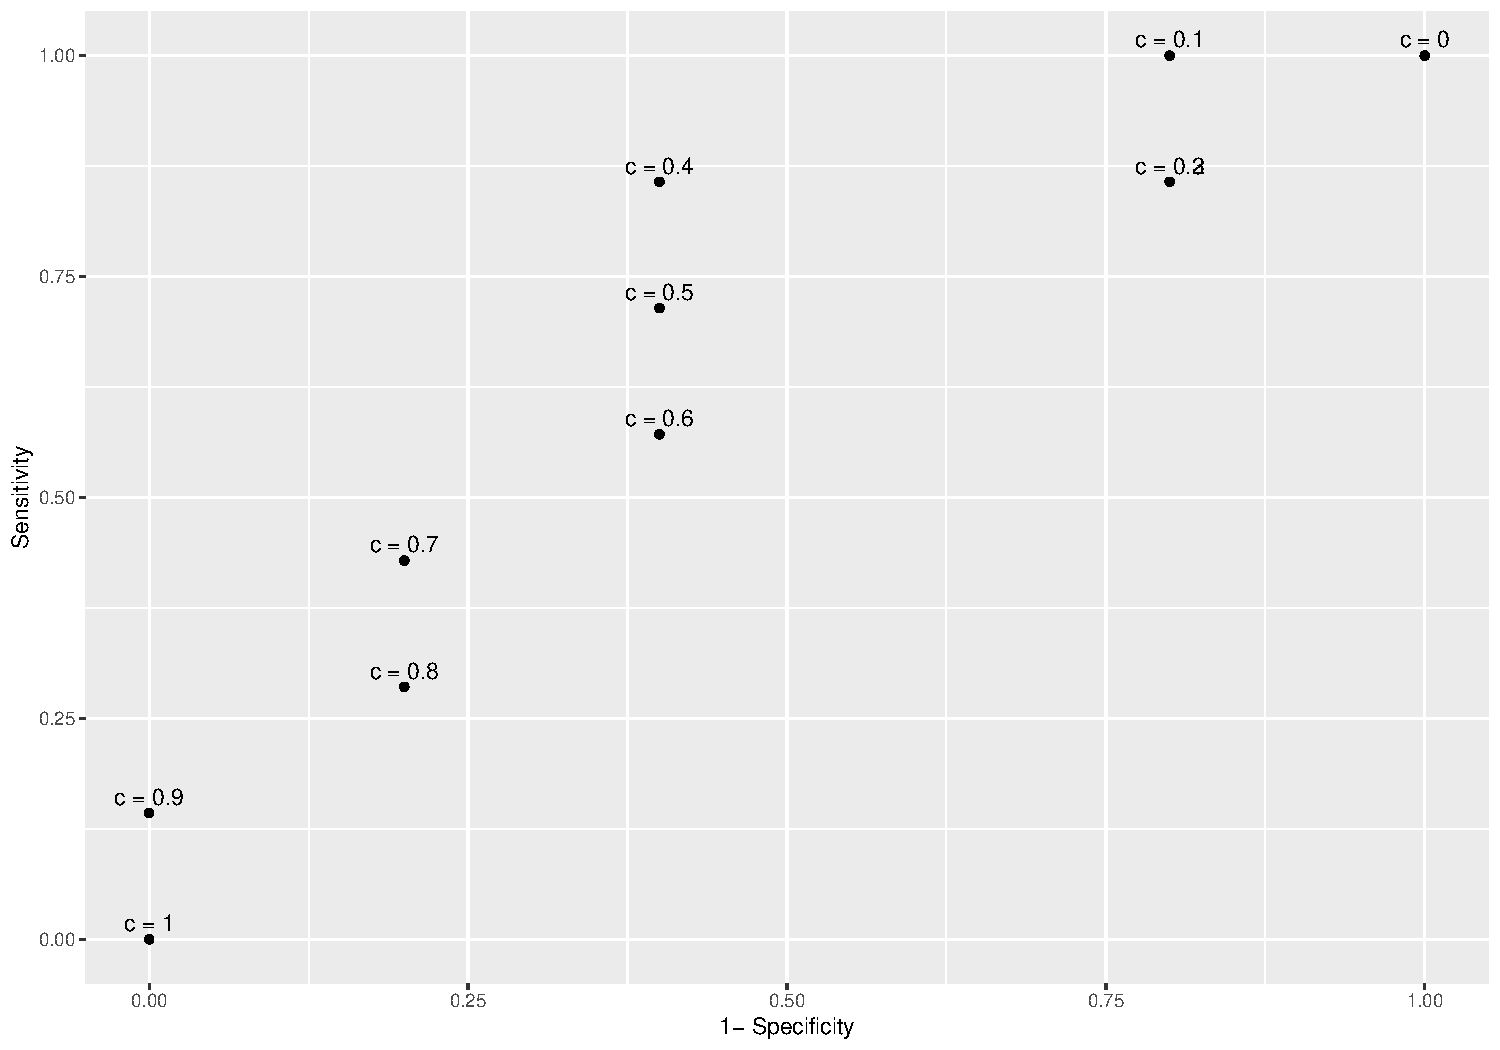
\includegraphics{measuring_performance_files/figure-beamer/unnamed-chunk-4-1.pdf}
\end{frame}

\begin{frame}{ROC Curve}
\protect\hypertarget{roc-curve}{}
\begin{itemize}
\tightlist
\item
  \textbf{Question}: What is the best cut-off value?
\item
  \textbf{Answer}: \(c = 0.4\) is the best cut-off value
\end{itemize}
\end{frame}

\begin{frame}{ROC Curve}
\protect\hypertarget{roc-curve-1}{}
\begin{itemize}
\tightlist
\item
  Each cut-off value \textbf{c} results a pair of (1-Specificity,
  Sensitivity) or (TP Rate, FP Rate)
\item
  The collections of all these pairs/points for all the cut-off values
  is the Receiver operating characteristic Curve (ROC Curve)
\end{itemize}
\end{frame}

\begin{frame}{ROC Curve of the example model}
\protect\hypertarget{roc-curve-of-the-example-model}{}
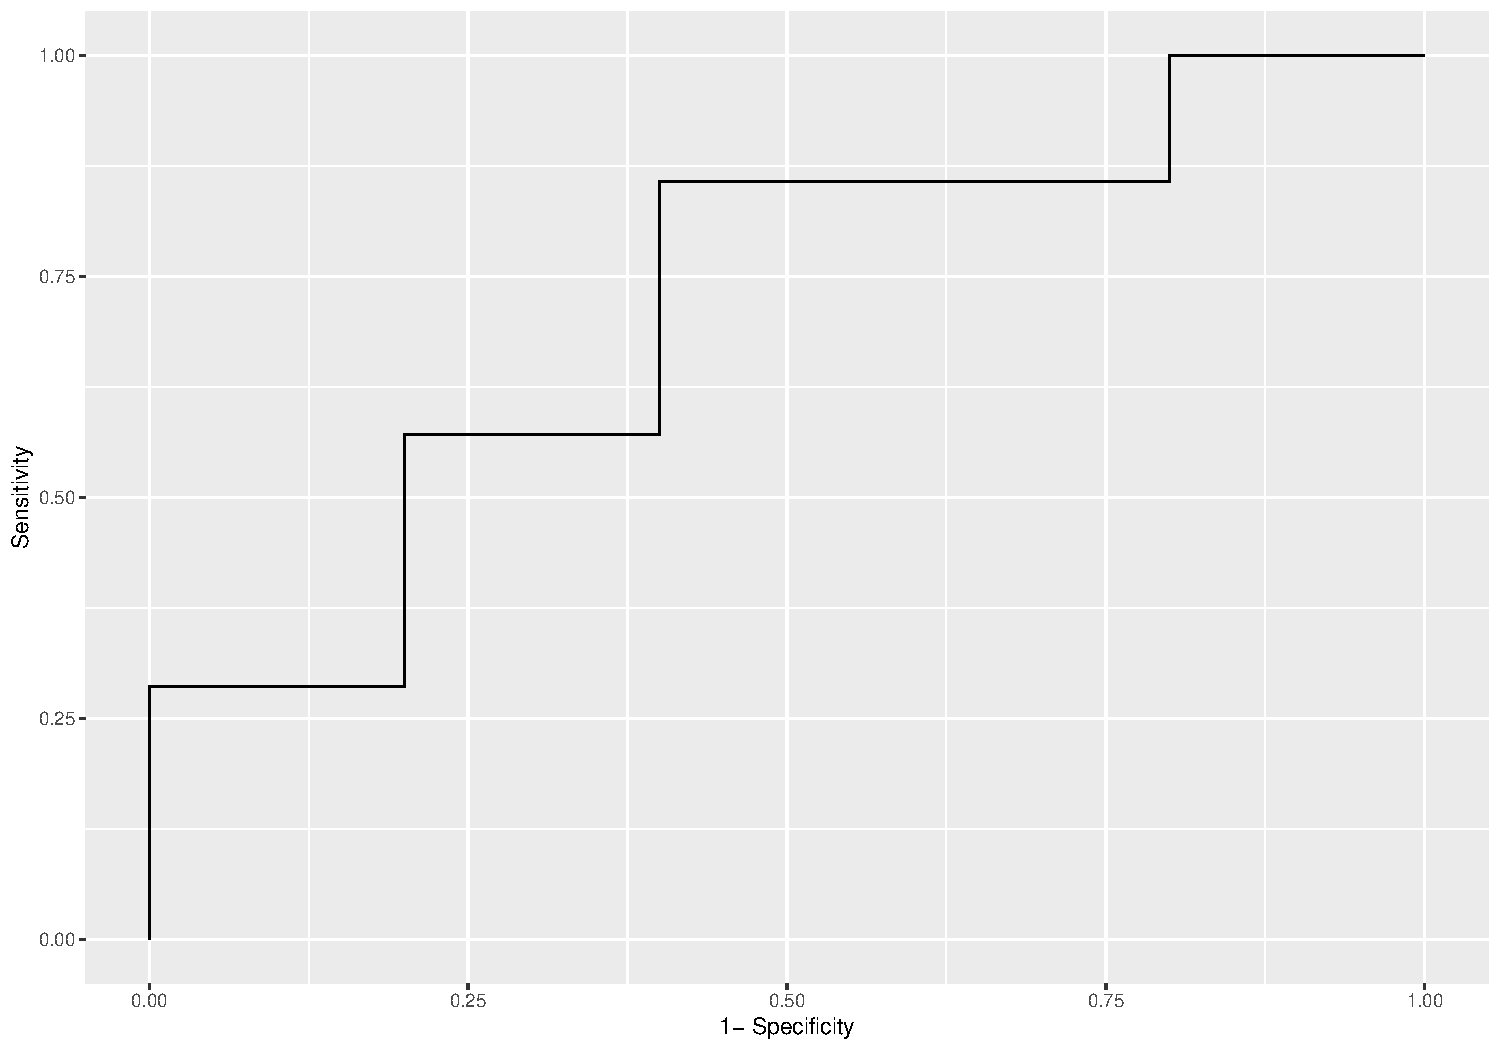
\includegraphics{measuring_performance_files/figure-beamer/unnamed-chunk-5-1.pdf}

\begin{itemize}
\tightlist
\item
  The curve is not very smooth because the data is very small
\item
  With bigger data, the ROC curve will be very ``smooth''
\end{itemize}
\end{frame}

\begin{frame}{ROC Curve}
\protect\hypertarget{roc-curve-2}{}
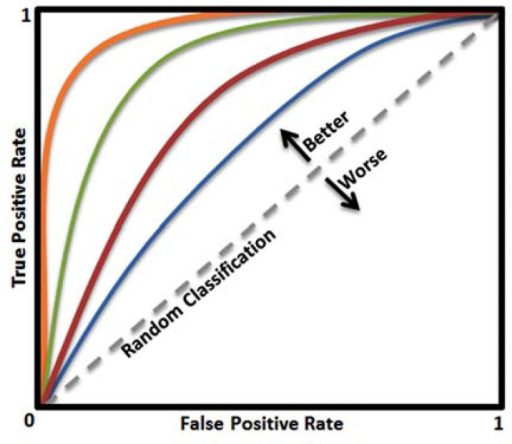
\includegraphics[width=3.125in,height=\textheight]{images/roc2.png}
\end{frame}

\begin{frame}{ROC Curve}
\protect\hypertarget{roc-curve-3}{}
\begin{itemize}
\tightlist
\item
  The closer the curve to the point (0,1) the better the model
\item
  The best cut-off value is at the point closest to (0,1)
\item
  (0,1) is the \textbf{perfect point}, resulting 0 misclassification
  model.\\
\item
  At (0,0) the model predicts everything positive
\item
  At (1,1) the model predicts everything negative
\item
  The ROC of the random guess model is the diagonal
\end{itemize}
\end{frame}

\begin{frame}{ROC Curve}
\protect\hypertarget{roc-curve-4}{}
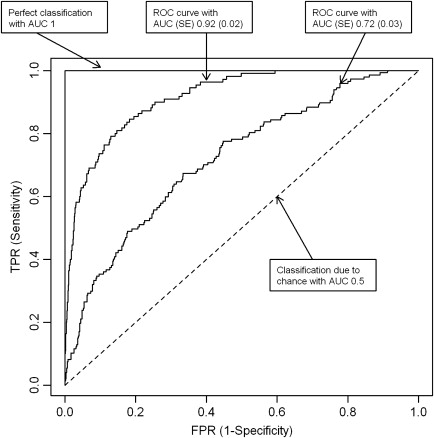
\includegraphics[width=3.125in,height=\textheight]{images/roc3.jpg}

\begin{itemize}
\tightlist
\item
  AUC = Area Under the (ROC) Curve
\end{itemize}
\end{frame}

\begin{frame}{ROC Curve}
\protect\hypertarget{roc-curve-5}{}
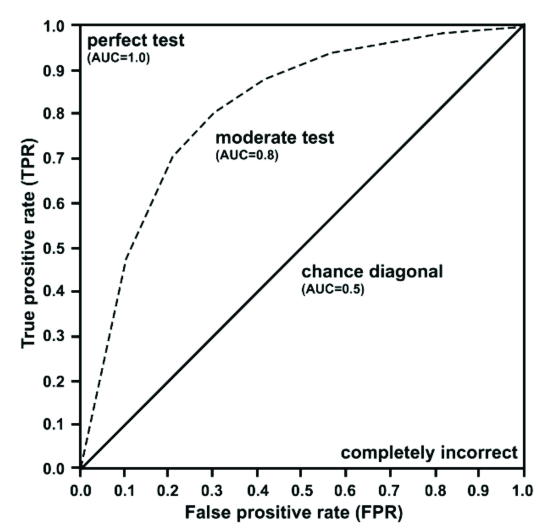
\includegraphics[width=3.125in,height=\textheight]{images/roc4.png}
\end{frame}

\begin{frame}{ROC Index}
\protect\hypertarget{roc-index}{}
\begin{itemize}
\tightlist
\item
  ROC Index is the area under the ROC Curve
\end{itemize}
\end{frame}

\begin{frame}{ROC Index - Area Under the Curve (AUC)}
\protect\hypertarget{roc-index---area-under-the-curve-auc}{}
\begin{itemize}
\item
  The closer the AUC to 1 the better the model
\item
  The closer the AUC to 1/2 the worse the model
\item
  Model with AUC = 1/2 is as good as a random guess or guessing by
  tossing a coin
\item
  \textbf{Question}: What if the AUC less than 1/2? Are models with AUC
  less than 1/2 \textbf{useless}?
\end{itemize}
\end{frame}

\begin{frame}{Another Question}
\protect\hypertarget{another-question}{}
\begin{itemize}
\tightlist
\item
  \textbf{Question}: Is the model with the misclassification rate of
  100\% the most \textbf{useless} model?
\end{itemize}
\end{frame}

\begin{frame}{Answer}
\protect\hypertarget{answer}{}
\begin{itemize}
\tightlist
\item
  \textbf{Question}: Is the model with the misclassification rate of
  100\% an useless model?
\item
  \emph{Answer}: No, by flipping the predictions of the models, one gets
  the \textbf{perfect model} with 0 misclassification rate.
\end{itemize}
\end{frame}

\begin{frame}{Back to the Question}
\protect\hypertarget{back-to-the-question}{}
\begin{itemize}
\item
  \textbf{Question}: What if the AUC less than 1/2? Are models with AUC
  less than 1/2 \textbf{useless}?
\item
  \textbf{Answer}: Model with AUC less than 1/2 could be made to be
  better by flipping the predictions (if the model predicts positve,
  flip it to predict negative)
\end{itemize}
\end{frame}

\begin{frame}{Cumulative Lift}
\protect\hypertarget{cumulative-lift}{}
\begin{itemize}
\tightlist
\item
  In the dataset, the ratio of ``Survived'' is 7/12 = 58.33\%
\item
  This mean that if we pick \textbf{randomly} a passenger in the this
  group, the chance of picking a ``Survived'' passenger is 58.33\%
\item
  \textbf{Question}: If we want to pick a ``Survived'' passenger, is
  there a better way than pick randomly?
\end{itemize}
\end{frame}

\begin{frame}{Cumulative Lift}
\protect\hypertarget{cumulative-lift-1}{}
\begin{itemize}
\tightlist
\item
  \textbf{Question}: If we want to pick a ``Survived'' passenger, is
  there a better way than pick randomly?
\item
  \textbf{Answer}: Yes, we should pick the one with the highest
  predictied probability.
\end{itemize}
\end{frame}

\begin{frame}{Cumulative Lift}
\protect\hypertarget{cumulative-lift-2}{}
\begin{longtable}[]{@{}rrr@{}}
\toprule
Order & Predicted Probabilities & True Values \\
\midrule
\endhead
1 & 0.94 & 1 \\
2 & 0.90 & 1 \\
3 & 0.84 & 0 \\
4 & 0.71 & 1 \\
5 & 0.68 & 1 \\
6 & 0.63 & 0 \\
7 & 0.55 & 1 \\
8 & 0.45 & 1 \\
9 & 0.38 & 0 \\
10 & 0.35 & 0 \\
11 & 0.20 & 1 \\
12 & 0.01 & 0 \\
\bottomrule
\end{longtable}

\begin{itemize}
\tightlist
\item
  Pick randomly, ``success rate'' is 58.33\%
\item
  Pick the top 1, success rate is 1/1 = 100\%
\item
  We say, at 1/12 = 8.33\%, the model lift is 100/58.33 = 1.71
\end{itemize}
\end{frame}

\begin{frame}{Cumulative Lift}
\protect\hypertarget{cumulative-lift-3}{}
\begin{longtable}[]{@{}rrr@{}}
\toprule
Order & Predicted Probabilities & True Values \\
\midrule
\endhead
1 & 0.94 & 1 \\
2 & 0.90 & 1 \\
3 & 0.84 & 0 \\
4 & 0.71 & 1 \\
5 & 0.68 & 1 \\
6 & 0.63 & 0 \\
7 & 0.55 & 1 \\
8 & 0.45 & 1 \\
9 & 0.38 & 0 \\
10 & 0.35 & 0 \\
11 & 0.20 & 1 \\
12 & 0.01 & 0 \\
\bottomrule
\end{longtable}

\begin{itemize}
\tightlist
\item
  Pick randomly, ``success rate'' is 58.33\%
\item
  Pick the top 2, success rate is 2/2 = 100\%
\item
  We say, at 2/12 = 16.67\%, the model lift is 100/58.33 = 1.71
\end{itemize}
\end{frame}

\begin{frame}{Cumulative Lift}
\protect\hypertarget{cumulative-lift-4}{}
\begin{longtable}[]{@{}rrr@{}}
\toprule
Order & Predicted Probabilities & True Values \\
\midrule
\endhead
1 & 0.94 & 1 \\
2 & 0.90 & 1 \\
3 & 0.84 & 0 \\
4 & 0.71 & 1 \\
5 & 0.68 & 1 \\
6 & 0.63 & 0 \\
7 & 0.55 & 1 \\
8 & 0.45 & 1 \\
9 & 0.38 & 0 \\
10 & 0.35 & 0 \\
11 & 0.20 & 1 \\
12 & 0.01 & 0 \\
\bottomrule
\end{longtable}

\begin{itemize}
\tightlist
\item
  Pick randomly, ``success rate'' is 58.33\%
\item
  Pick the top 2, success rate is 2/2 = 100\%
\item
  We say, at 2/12 = 16.67\%, the model lift is 100/58.33 = 1.71
\end{itemize}
\end{frame}

\begin{frame}{Cumulative Lift}
\protect\hypertarget{cumulative-lift-5}{}
\begin{longtable}[]{@{}rrr@{}}
\toprule
Order & Predicted Probabilities & True Values \\
\midrule
\endhead
1 & 0.94 & 1 \\
2 & 0.90 & 1 \\
3 & 0.84 & 0 \\
4 & 0.71 & 1 \\
5 & 0.68 & 1 \\
6 & 0.63 & 0 \\
7 & 0.55 & 1 \\
8 & 0.45 & 1 \\
9 & 0.38 & 0 \\
10 & 0.35 & 0 \\
11 & 0.20 & 1 \\
12 & 0.01 & 0 \\
\bottomrule
\end{longtable}

\begin{itemize}
\tightlist
\item
  Pick randomly, ``success rate'' is 58.33\%
\item
  Pick the top 3, success rate is 2/3 = 66.66\%
\item
  We say, at 3/12 = 25\%, the model lift is 66.66/58.33 = 1.14
\end{itemize}
\end{frame}

\begin{frame}{Cumulative Lift}
\protect\hypertarget{cumulative-lift-6}{}
\begin{longtable}[]{@{}rrr@{}}
\toprule
Order & Predicted Probabilities & True Values \\
\midrule
\endhead
1 & 0.94 & 1 \\
2 & 0.90 & 1 \\
3 & 0.84 & 0 \\
4 & 0.71 & 1 \\
5 & 0.68 & 1 \\
6 & 0.63 & 0 \\
7 & 0.55 & 1 \\
8 & 0.45 & 1 \\
9 & 0.38 & 0 \\
10 & 0.35 & 0 \\
11 & 0.20 & 1 \\
12 & 0.01 & 0 \\
\bottomrule
\end{longtable}

\begin{itemize}
\tightlist
\item
  Pick randomly, ``success rate'' is 58.33\%
\item
  Pick the top 4, success rate is 3/4 = 75\%
\item
  We say, at 4/12 = 25\%, the model lift is 75/58.33 = 1.28
\end{itemize}
\end{frame}

\begin{frame}{Cumulative Lift}
\protect\hypertarget{cumulative-lift-7}{}
\begin{longtable}[]{@{}rr@{}}
\toprule
Percentage & Lift \\
\midrule
\endhead
0.0833333 & 1.714286 \\
0.1666667 & 1.714286 \\
0.2500000 & 1.142857 \\
0.3333333 & 1.285714 \\
0.4166667 & 1.371429 \\
0.5000000 & 1.142857 \\
0.5833333 & 1.224490 \\
0.6666667 & 1.285714 \\
0.7500000 & 1.142857 \\
0.8333333 & 1.028571 \\
0.9166667 & 1.090909 \\
1.0000000 & 1.000000 \\
\bottomrule
\end{longtable}
\end{frame}

\begin{frame}{Cumulative Lift}
\protect\hypertarget{cumulative-lift-8}{}
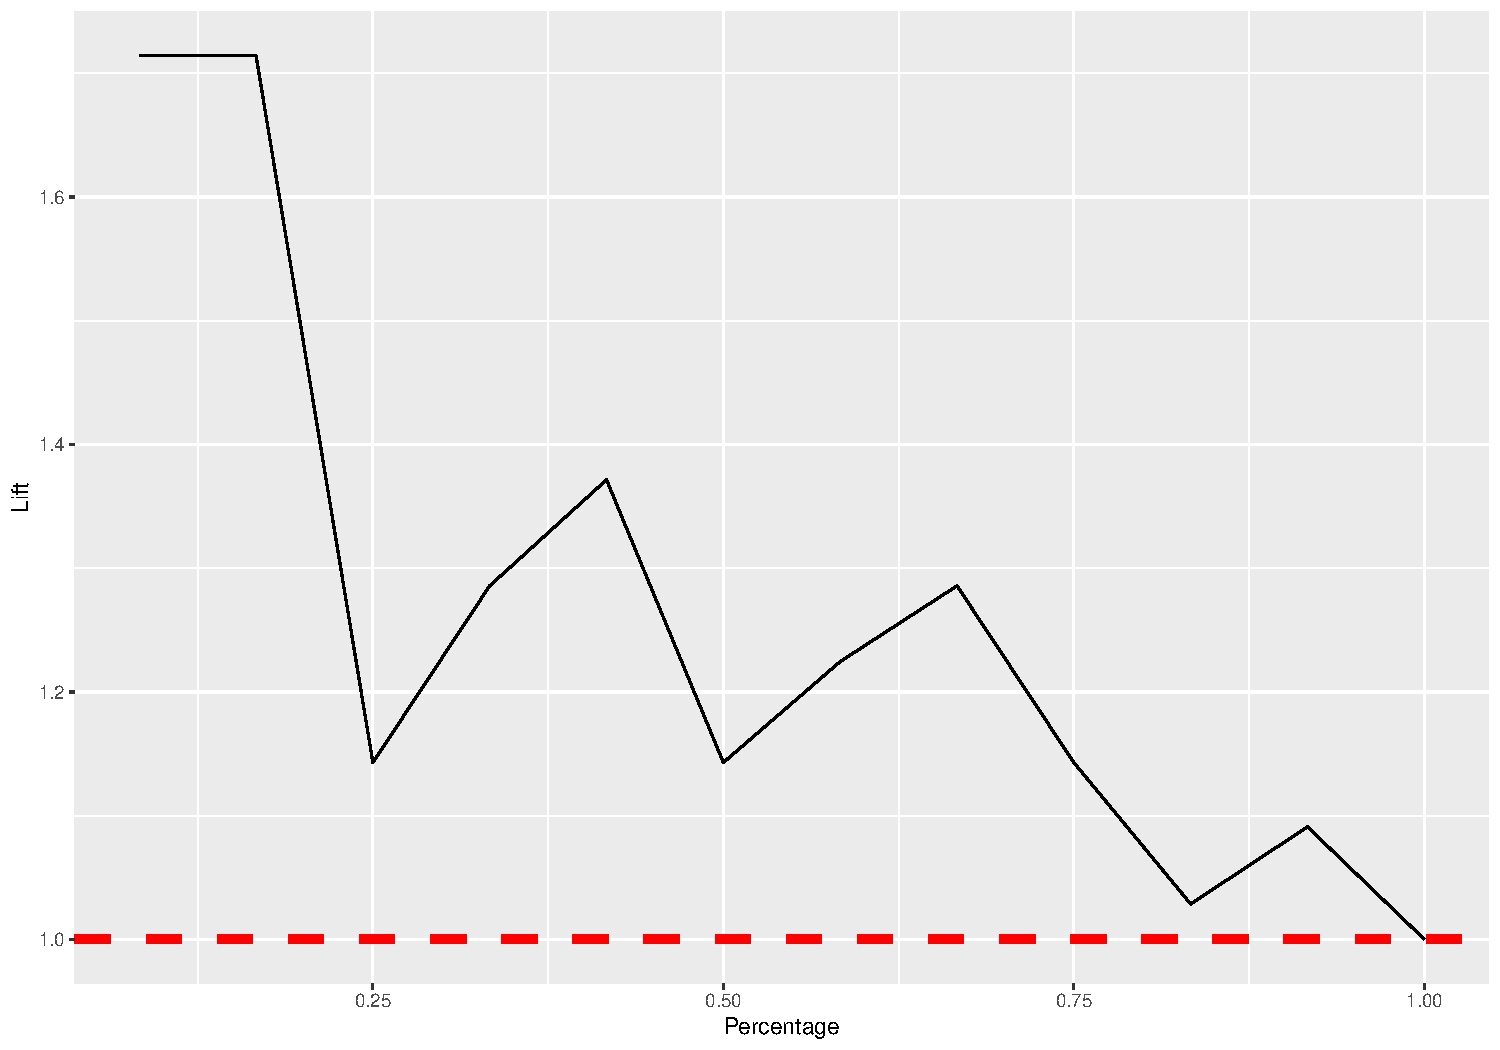
\includegraphics{measuring_performance_files/figure-beamer/unnamed-chunk-12-1.pdf}
\end{frame}

\begin{frame}{Cumulative \% Response}
\protect\hypertarget{cumulative-response}{}
\begin{longtable}[]{@{}rr@{}}
\toprule
Percentage & Percent\_Response \\
\midrule
\endhead
0.0833333 & 1.0000000 \\
0.1666667 & 1.0000000 \\
0.2500000 & 0.6666667 \\
0.3333333 & 0.7500000 \\
0.4166667 & 0.8000000 \\
0.5000000 & 0.6666667 \\
0.5833333 & 0.7142857 \\
0.6666667 & 0.7500000 \\
0.7500000 & 0.6666667 \\
0.8333333 & 0.6000000 \\
0.9166667 & 0.6363636 \\
1.0000000 & 0.5833333 \\
\bottomrule
\end{longtable}
\end{frame}

\begin{frame}{Cumulative \% Response}
\protect\hypertarget{cumulative-response-1}{}
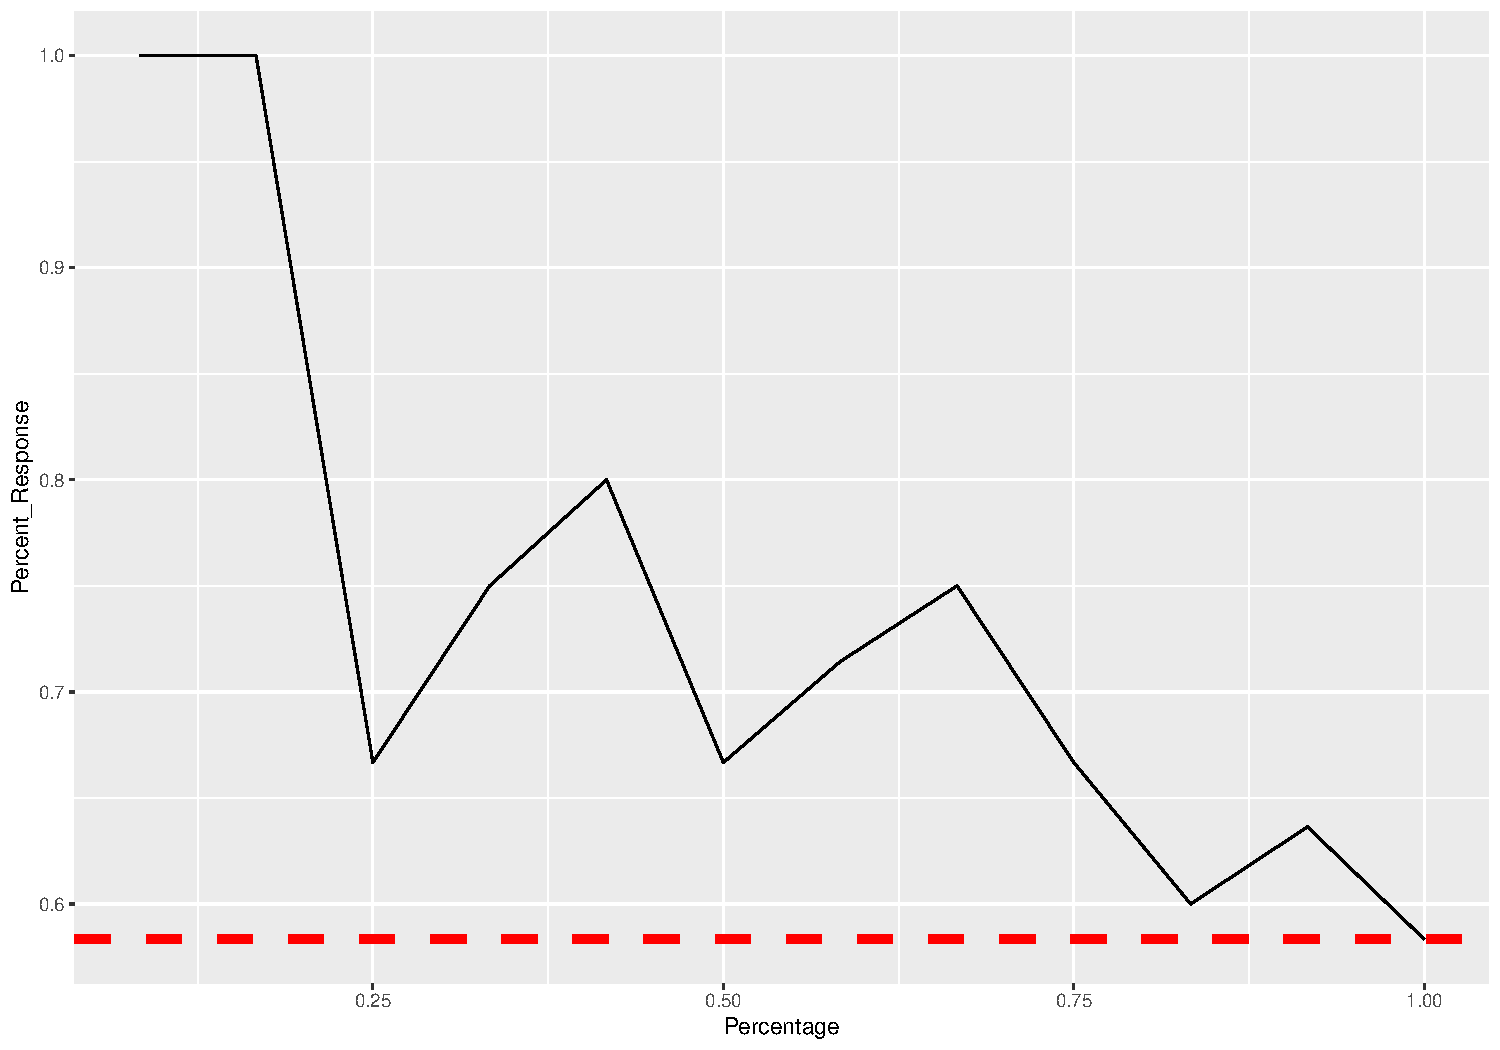
\includegraphics{measuring_performance_files/figure-beamer/unnamed-chunk-14-1.pdf}
\end{frame}

\end{document}
